%%%%%% CMB-S4 Simulations and Data Analysis Chapter, Data Simulation Section  %%%%%%%%%%%%%%%%
 
\section{Data Simulation}

\begin{figure}[htbp]
\centering
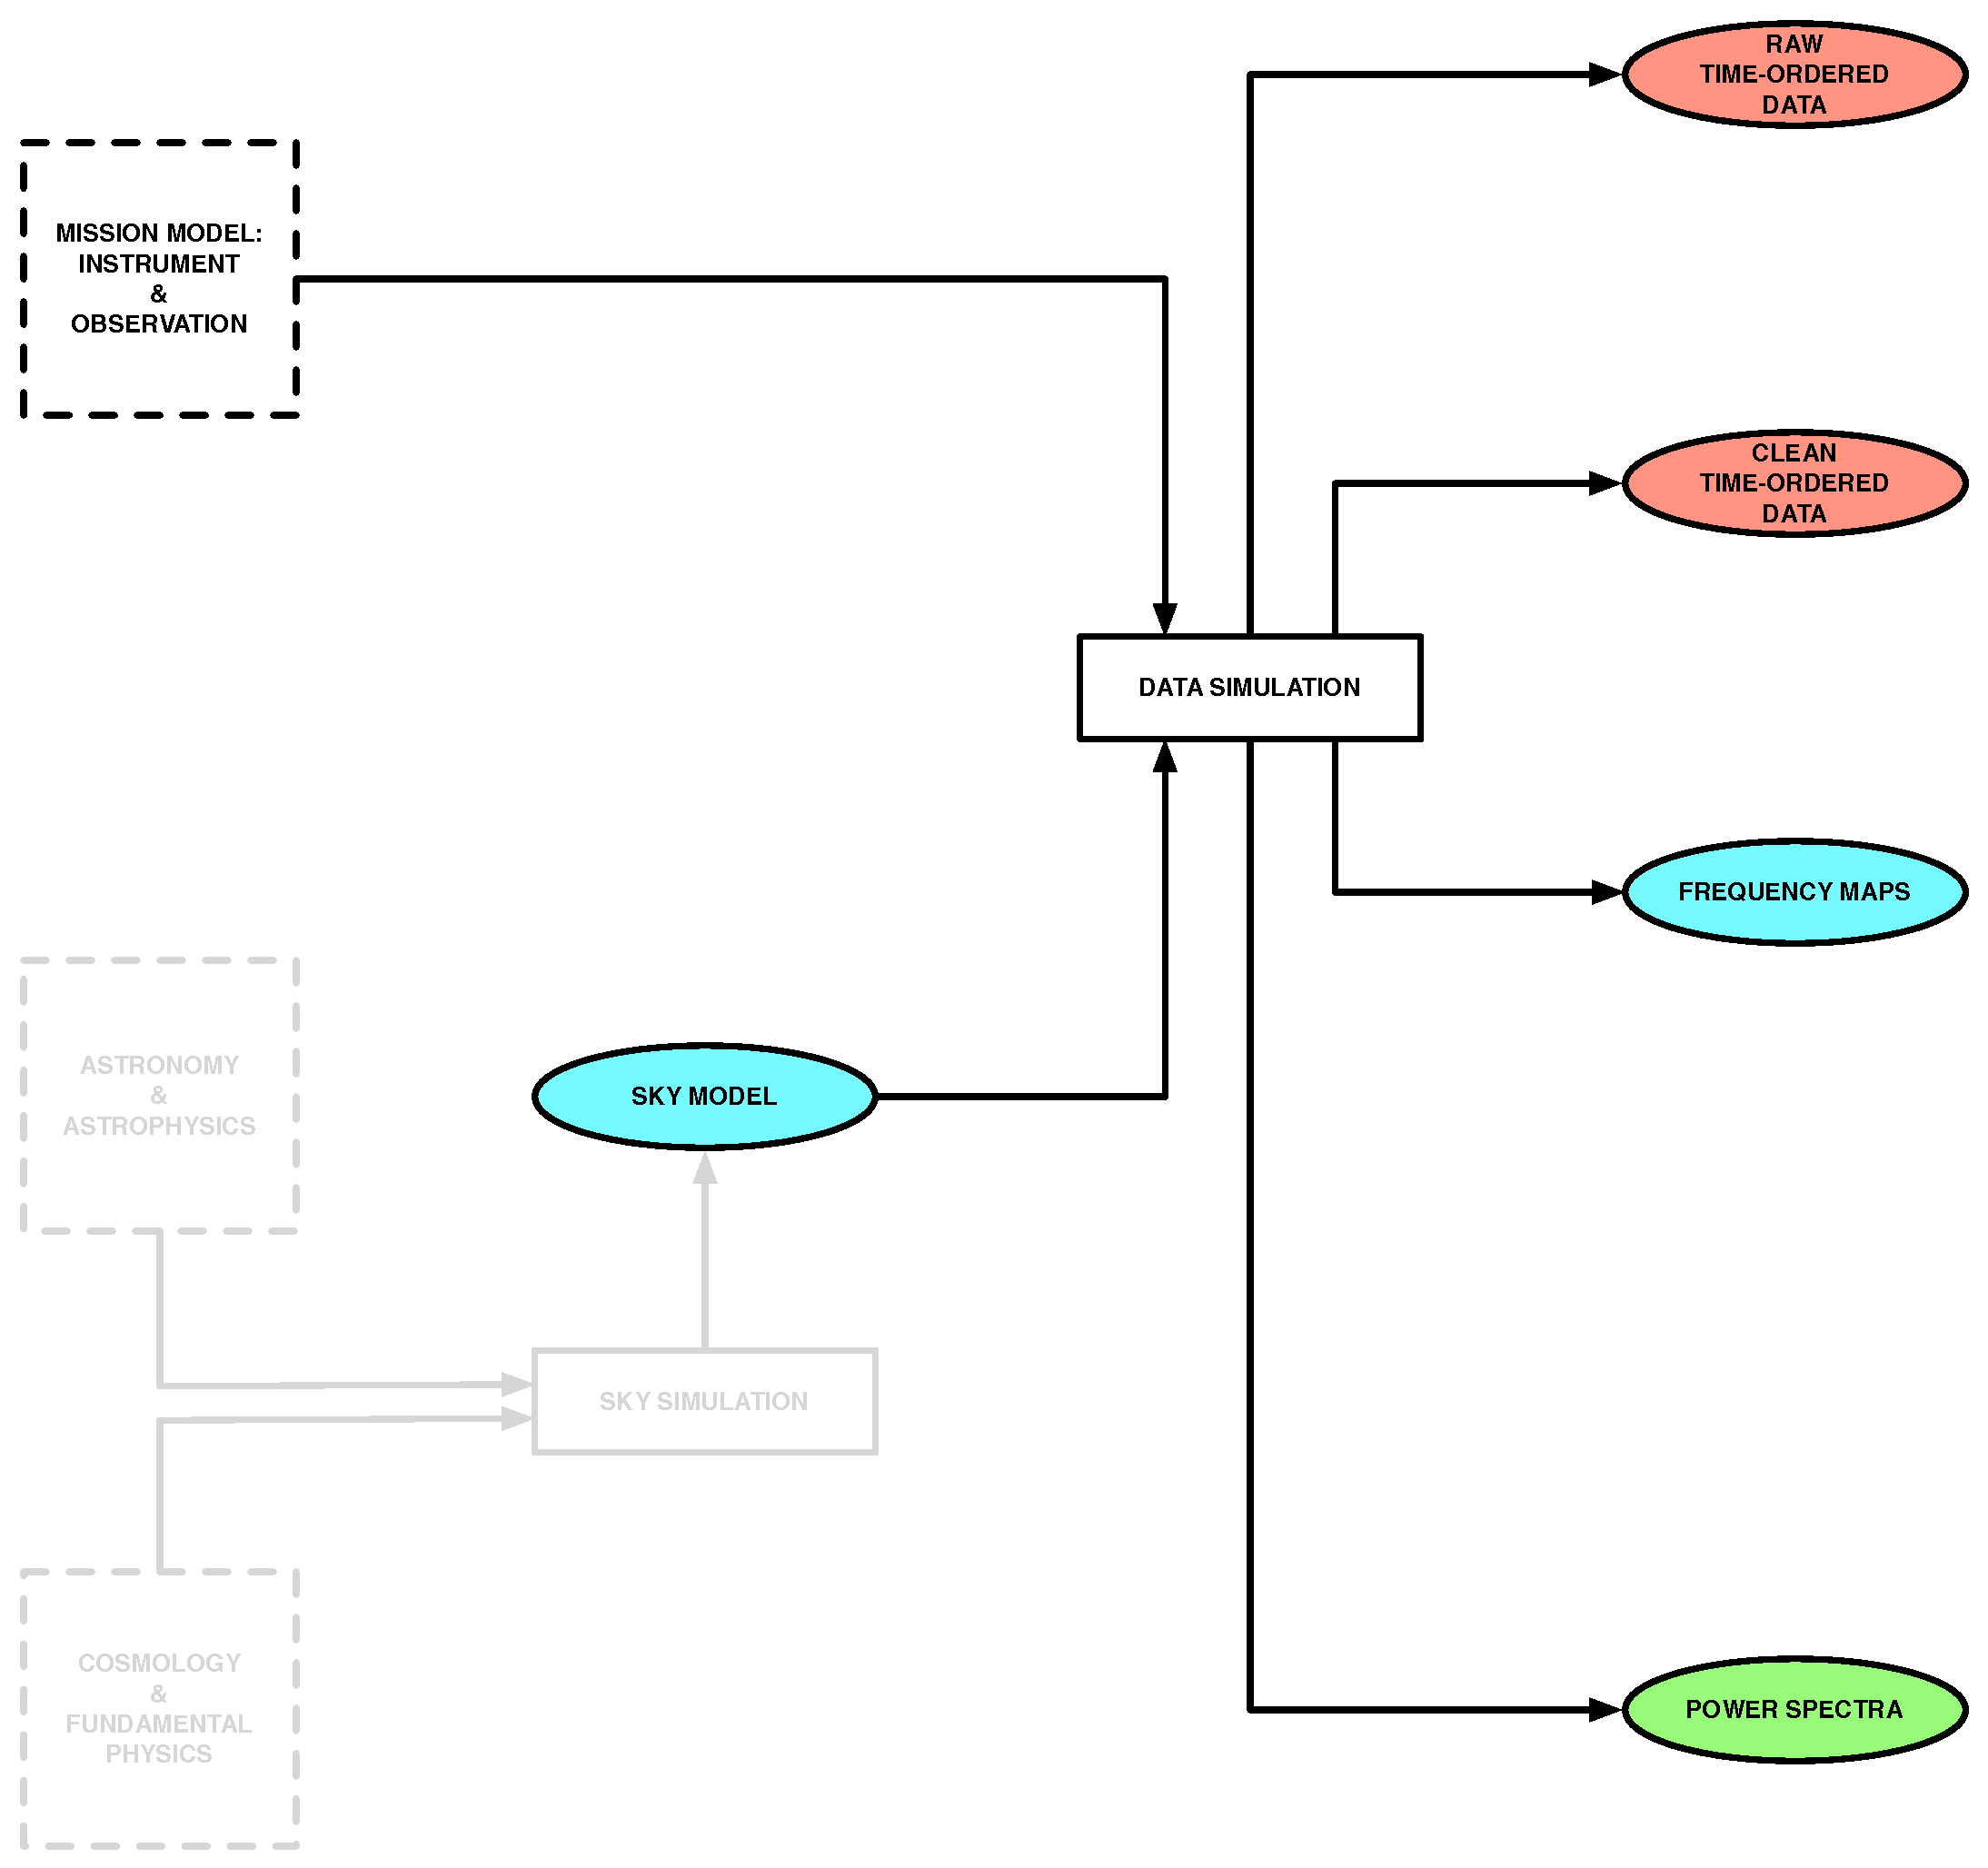
\includegraphics[width=1\textwidth]{Analysis/ds}
\caption{The data simulation subset of the CMB simulation pipeline}
\label{fig:skymodel-in-pipeline}
\end{figure}


Sky model

Mission model:

Instrument - beam, bandpass, hwp, detector/readout electronics

Observation - pointing, flagging, atmosphere, ground

\subsection{Time Domain}

\subsubsection{Raw TOD}

The simulation of detector-level time ordered data serves a number of purposes, including 1.  end-to-end analysis pipeline validation, 2.  propagation of instrument systematic errors to errors in science results.  The software tool will be flexible enough to easily accommodate modifications as the instrument is better characterized with operational experience.  The software will be modular so that levels of complexity can be included or skipped, depending on the requirements of a particular simulation task.

A sky resampler reads the predicted astrophysical sky signal from a sky model map convolved with a beam shape and bandpass model for a given detector pointing.  The astrophysical sky signal is added to additional simulated signals from stray light, atmospheric signal fluctuations, and ground pickup.  The signal is propagated through a simple simulation of the optics to include polarization angle rotations and optical efficiencies of the optical stages. This results in a simulated  time ordered data set of the total millimeter-wave power incident on the detector.

A physical model of the detector system and associated readout is used to convert the simulated optical power into detector output that is designed to mimic  the response of the instrument to the incident optical power, both from sky signal and other sources. The details of the physical model depend on the detector technology chosen for a given band, but as an example case, consider a transition-edge superconducting (TES) bolometer read out with multiplexed SQUID amplifiers.  The simulator would model the flow of heat in the TES absorber and the flow of current and magnetic flux through the SQUID readout.  Variations in ambient magnetic field could be added at this stage.  The simulator would require the concurrent simulation of multiple detectors using the same multiplex channel so as to include correlations induced by crosstalk or thermal fluctuations.  Additional filters applied by the readout electronics would also be included, including digitization with an analog to digital converter. For MKID or coherent receivers, the physical model would be different in detail, but would include a similarly detailed model in order to easily allow systematic error injection anywhere in the system.

\subsubsection{Clean TOD}

Effective beam convolution (map domain via time domain pointing)

%% Map/spectral domain text lifted from forecasting section?

\subsection{Map Domain}

\subsection{Spectral Domain}

%\bibliography{cmbs4}

%%
%% Populate the .bib file with entries from SPIRES Bibtex (preferred)
%% or ADS Bibtex (if no SPIRES entry).
%%  SPIRES will also supply the CITATION line information; please include it.
%%


